\chapter{Anexo: WebGPU y Machine Learning en el Navegador}
\label{anexo-webgpu}

Este anexo explora WebGPU, una tecnología emergente que permite la ejecución eficiente de modelos de Machine Learning directamente en el navegador web, y su impacto en el desarrollo de aplicaciones web modernas.

\begin{figure}[H]
    \centering
    
\includegraphics[width=0.4\textwidth]{figuras/webgpu.png}
    \caption{Logo de WebGPU}
    \label{fig:webgpu-logo}
\end{figure}

WebGPU representa la nueva generación de APIs gráficas para la web, sucediendo a WebGL como el estándar para computación de alto rendimiento en navegadores. A diferencia de sus predecesores, WebGPU está diseñado desde cero para aprovechar las arquitecturas modernas de GPU y proporcionar acceso a capacidades de computación general.

\section{Características Principales}
\begin{itemize}
    \item \textbf{Compute Shaders}: Permite la ejecución de código de propósito general en la GPU, fundamental para operaciones de ML.
    \item \textbf{Gestión de Memoria Explícita}: Mayor control sobre la asignación y liberación de memoria en la GPU.
    \item \textbf{Pipeline de Renderizado Moderno}: Arquitectura basada en comandos que reduce la sobrecarga del driver.
    \item \textbf{Mejor Paralelismo}: Aprovecha eficientemente los núcleos de la GPU para computación paralela.
\end{itemize}


\section{Arquitectura General de WebGPU}
\label{sec:webgpu-architecture}

WebGPU proporciona una interfaz moderna y eficiente para acceder a las capacidades de computación de la GPU. Esta sección detalla su arquitectura general y los componentes principales que permiten la ejecución eficiente de tareas de computación paralela.

\subsection{Componentes Principales}
\label{subsec:main-components}

\subsubsection{Dispositivo Lógico (GPUDevice)}
El \texttt{GPUDevice} representa una interfaz lógica al hardware GPU y gestiona todos los recursos y operaciones. La inicialización se realiza con:
\begin{equation}
    \text{device} = \text{await adapter.requestDevice(descriptor);}
\end{equation}
El dispositivo gestiona capacidades como límites de recursos, configuraciones de pipeline y formatos de memoria.

\subsubsection{Sistema de Recursos}
Los recursos son las unidades básicas de almacenamiento y procesamiento. Los principales tipos son:
\begin{itemize}
    \item \textbf{GPUBuffer}: Almacenamiento lineal de datos, con tipos de uso como Storage, Uniform, Vertex, e Index. Permite mapeo de memoria para transferencia CPU-GPU.
    \item \textbf{GPUTexture}: Almacenamiento optimizado para datos 2D/3D, con soporte para mipmapping y sampling.
\end{itemize}

\subsection{Pipeline de Computación}
\label{subsec:compute-pipeline}

El pipeline define cómo se procesan los datos. La creación del pipeline se realiza con:
\begin{equation}
    \text{pipeline} = \text{device.createComputePipeline(descriptor);}
\end{equation}
Los componentes incluyen el Shader Module (código WGSL), el Layout (descripción de recursos y bindings) y el Entry Point (punto de entrada para la ejecución).

\subsection{Sistema de Comandos}
\label{subsec:command-system}

La ejecución se gestiona mediante un sistema de comandos, compuesto por:
\begin{itemize}
    \item \textbf{Command Encoder}: Creación y registro de comandos, configuración de estados y recursos, y definición de pases de computación.
    \item \textbf{Command Queue}: Cola de comandos para ejecución, sincronización de operaciones y gestión de dependencias.
\end{itemize}

\subsection{Flujo de Ejecución}
\label{subsec:execution-flow}

El proceso típico de ejecución sigue estos pasos:
\begin{enumerate}
    \item \textbf{Inicialización}: Obtención del adaptador GPU, creación del dispositivo lógico y configuración de recursos iniciales.
    \item \textbf{Preparación de Recursos}: Creación de buffers y texturas, carga de datos desde CPU y configuración de bind groups.
    \item \textbf{Configuración de Pipeline}: Compilación de shaders, definición de layouts y configuración de estados.
    \item \textbf{Ejecución}: Codificación de comandos, submisión a la cola y sincronización y espera de resultados.
\end{enumerate}

\subsection{Optimizaciones}
\label{subsec:optimizations}

Para mejorar el rendimiento, se pueden aplicar las siguientes optimizaciones:
\begin{itemize}
    \item \textbf{Gestión de Memoria}: Buffer pooling y reutilización, estrategias de paginación, alineación y padding óptimos.
    \item \textbf{Paralelismo}: Optimización de workgroups, overlapping de pipelines y submisión asíncrona de comandos.
    \item \textbf{Sincronización}: Sincronización con fences, coordinación basada en eventos y barreras de memoria.
\end{itemize}

\subsection{Consideraciones de Rendimiento}
\label{subsec:performance-considerations}

Para maximizar el rendimiento, se deben considerar:
\begin{itemize}
    \item \textbf{Latencia}: Minimización de transferencias CPU-GPU, procesamiento en batch y reutilización de command buffers.
    \item \textbf{Throughput}: Optimización de patrones de acceso a memoria, balanceo de carga entre workgroups y optimización del estado del pipeline.
\end{itemize}

\section{Diagrama de Arquitectura WebGPU}
\label{sec:webgpu-architecture-diagram}

La Figura~\ref{fig:webgpu-architecture} presenta la arquitectura general de WebGPU, ilustrando la relación entre sus diferentes componentes y el flujo de datos desde la aplicación hasta el hardware GPU. La arquitectura se divide en tres capas principales que facilitan la ejecución eficiente de operaciones de computación paralela en el navegador.

\begin{figure}[H]
    \centering
    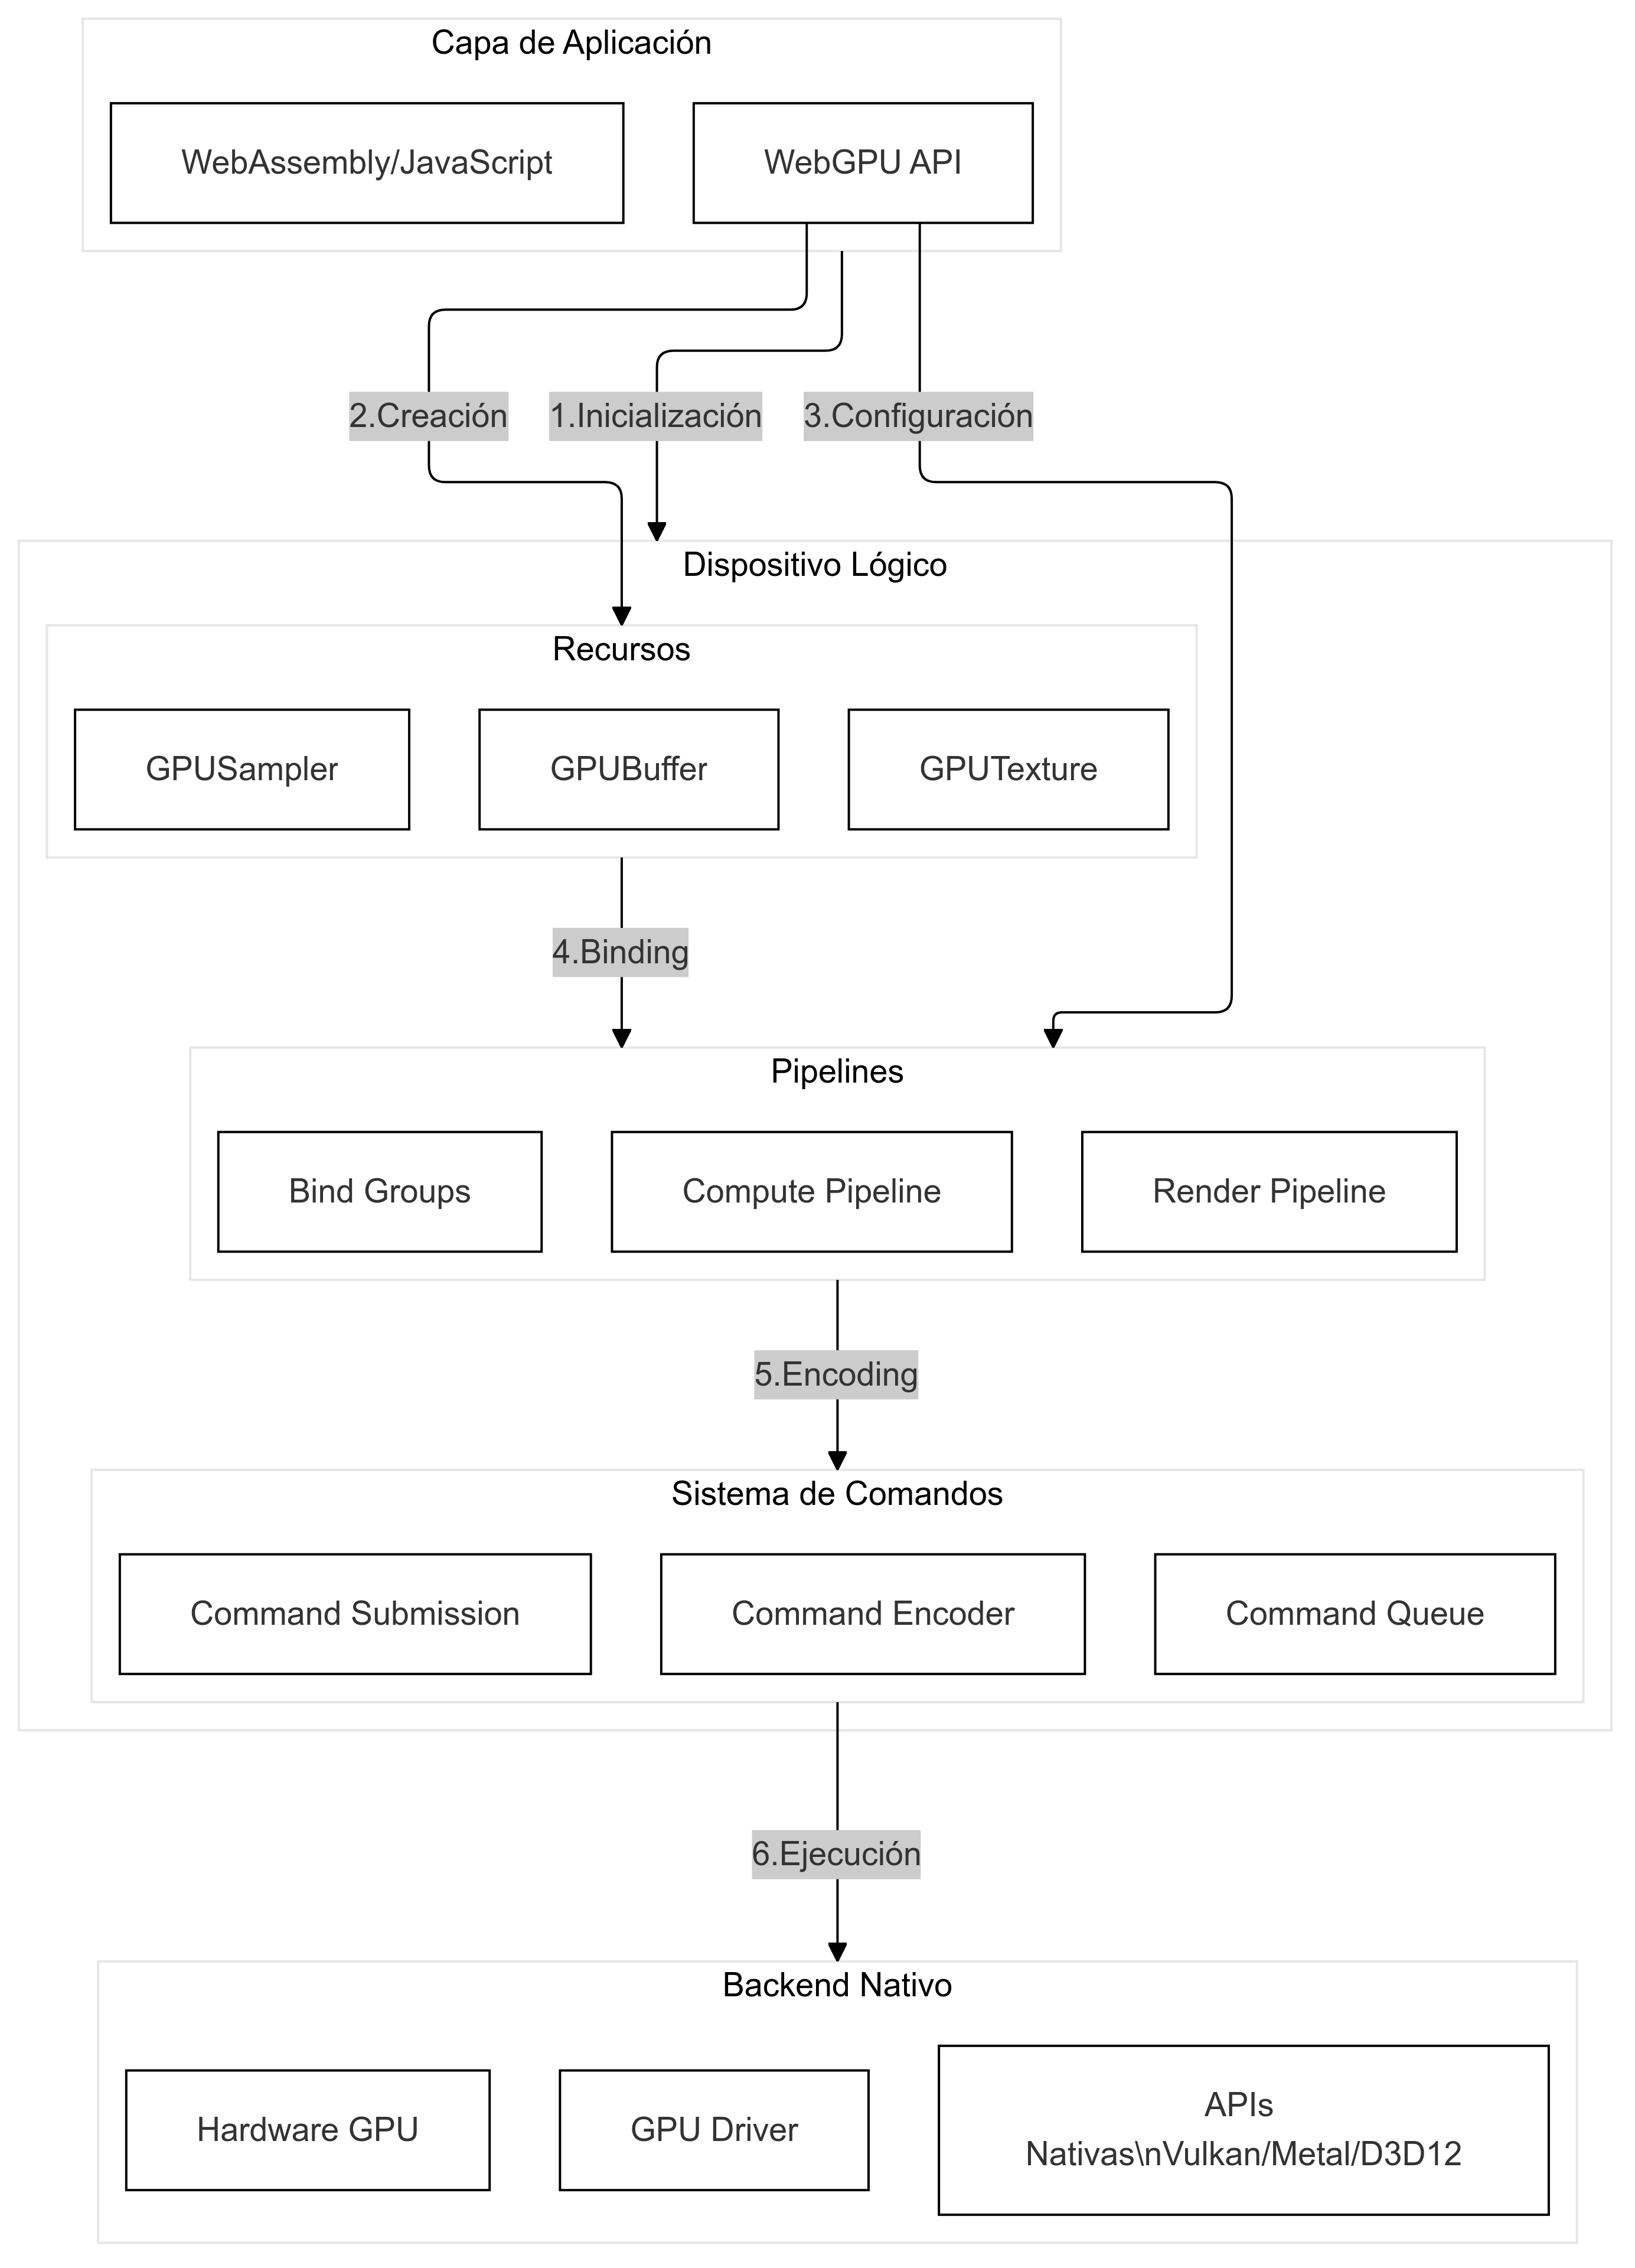
\includegraphics[width=0.8\textwidth]{figuras/webgpu-architecture.png}
    \caption{Arquitectura general de WebGPU y flujo de datos}
    \label{fig:webgpu-architecture}
\end{figure}




\subsection{Estructura de Capas}
\label{subsec:layer-structure}

\begin{itemize}
    \item \textbf{Capa de Aplicación}:
    \begin{itemize}
        \item WebAssembly/JavaScript para la interfaz de programación
        \item WebGPU API para la configuración y control de operaciones
    \end{itemize}

    \item \textbf{Dispositivo Lógico}:
    \begin{itemize}
        \item \texttt{Recursos}: Gestión de buffers, texturas y samplers para datos
        \item \texttt{Pipelines}: Configuración de operaciones de computación y renderizado
        \item \texttt{Sistema de Comandos}: Codificación y control de ejecución
    \end{itemize}

    \item \textbf{Backend Nativo}:
    \begin{itemize}
        \item Driver GPU y APIs nativas (Vulkan/Metal/D3D12)
        \item Conexión directa con el hardware para ejecución
    \end{itemize}
\end{itemize}

\subsection{Flujo de Operación}
\label{subsec:operation-flow}

El proceso de ejecución sigue una secuencia definida:

\begin{enumerate}
    \item \textbf{Inicialización}: La aplicación inicializa el dispositivo GPU.
    \item \textbf{Creación}: La API de WebGPU crea los recursos necesarios (buffers, texturas, samplers).
    \item \textbf{Configuración}: Se establecen los pipelines de computación y renderizado.
    \item \textbf{Binding}: Los recursos se vinculan a los pipelines mediante bind groups.
    \item \textbf{Encoding}: Los pipelines configurados generan comandos mediante el encoder.
    \item \textbf{Ejecución}: Los comandos codificados se ejecutan en el hardware a través del backend nativo.
\end{enumerate}

Esta arquitectura permite una gestión eficiente de recursos y operaciones, facilitando la ejecución de tareas complejas como procesamiento de audio, video y modelos de machine learning directamente en el navegador. La separación en capas proporciona una base sólida para optimizaciones y facilita el mantenimiento del código.

\section{Rendimiento y Benchmarks}

\subsection{Comparativa entre WebGPU y WebGL}

WebGPU representa la siguiente generación de APIs gráficas para la web, diseñada como sucesor de WebGL. Mientras que WebGL se basó en OpenGL ES, proporcionando una API gráfica para la web, WebGPU ha sido diseñado desde cero para aprovechar las arquitecturas GPU modernas y proporcionar acceso a capacidades de computación más avanzadas. La Tabla~\ref{tab:webgpu-webgl} presenta las diferencias técnicas más significativas entre ambas tecnologías, destacando las mejoras fundamentales que WebGPU introduce en términos de rendimiento, control y capacidades de computación.

\label{sec:webgpu-webgl-comparison}

\begin{table}[H]
\caption{Diferencias técnicas principales entre WebGPU y WebGL}
\label{tab:webgpu-webgl}
\begin{tabular}{|p{3cm}|p{5cm}|p{5cm}|}
\hline
\textbf{Característica} & \textbf{WebGPU} & \textbf{WebGL} \\
\hline
\textbf{Modelo de Ejecución} & 
Multi-thread con async compute y ejecución paralela de comandos & 
Single-thread con sincronización bloqueante \\
\hline
\textbf{Gestión de Memoria} & 
Control explícito con buffer pooling y mapeo directo de memoria GPU & 
Gestión implícita a través del driver OpenGL con overhead adicional \\
\hline
\textbf{Pipeline} & 
Pipeline basado en comandos con compute shaders y control granular de estados & 
Pipeline fijo con estados globales y sin soporte nativo para compute shaders \\
\hline
\textbf{APIs Backend} & 
APIs modernas (Vulkan/Metal/D3D12) con acceso directo al hardware y menor overhead & 
OpenGL/OpenGL ES con múltiples capas de abstracción y mayor latencia \\
\hline
\textbf{Capacidades de Computación} & 
Soporte nativo para GPGPU, procesamiento tensorial y operaciones atómicas & 
Limitado a operaciones gráficas, sin soporte para computación general \\
\hline
\end{tabular}
\end{table}

\subsection{Comparativa de Experiencia de Usuario: WebGPU vs Backend}
\label{sec:webgpu-backend-comparison}

La elección entre procesamiento local mediante WebGPU y procesamiento en backend impacta significativamente en la experiencia del usuario final. Esta comparativa analiza los aspectos clave que afectan directamente a la interacción del usuario con la aplicación, considerando factores como latencia, privacidad y disponibilidad de recursos.

\begin{table}[H]
\caption{Comparación de experiencia de usuario entre WebGPU y Backend}
\label{tab:webgpu-backend-ux}
\begin{tabular}{|p{3cm}|p{5cm}|p{5cm}|}
\hline
\textbf{Aspecto} & \textbf{WebGPU (Local)} & \textbf{Backend} \\
\hline
\textbf{Latencia} & 
Respuesta inmediata sin depender de la conexión a internet & 
Latencia variable dependiente de la conexión y carga del servidor \\
\hline
\textbf{Privacidad} & 
Datos procesados localmente sin salir del dispositivo & 
Datos enviados y procesados en servidores externos \\
\hline
\textbf{Disponibilidad} & 
Funciona offline una vez cargados los modelos & 
Requiere conexión constante a internet \\
\hline
\textbf{Recursos} & 
Limitado por el hardware del dispositivo del usuario & 
Acceso a recursos computacionales escalables \\
\hline
\textbf{Consistencia} & 
Rendimiento consistente basado en el dispositivo del usuario & 
Rendimiento variable según carga del servidor y red \\
\hline
\end{tabular}
\end{table}

\section{Futuro y Evolución}
\label{sec:future-evolution}

WebGPU representa un cambio significativo en la computación web, y su evolución continúa marcando el camino hacia nuevas posibilidades en el procesamiento GPU en el navegador. Esta sección explora las direcciones futuras y el impacto potencial de esta tecnología.

\subsection{Avances Técnicos Previstos}
\label{subsec:technical-advances}

\subsubsection{Operaciones Tensoriales}
El futuro de WebGPU en el ámbito del Machine Learning se centra en la implementación de operaciones tensoriales altamente optimizadas. Se están desarrollando aceleradores específicos para redes neuronales y mejorando el soporte para tipos de datos de precisión mixta. Estas optimizaciones serán particularmente relevantes para la ejecución eficiente de modelos de lenguaje grandes en el navegador.

\subsubsection{Interoperabilidad}
Se prevé una integración más profunda con las APIs web existentes y una mejor compatibilidad con formatos de modelos estándar. Las futuras versiones de WebGPU incluirán interfaces unificadas para el procesamiento multimedia y mejorarán la conectividad con sistemas de visualización avanzada, facilitando el desarrollo de aplicaciones web más sofisticadas.

\subsubsection{Optimizaciones de Rendimiento}
Las próximas iteraciones de WebGPU se centrarán en mejorar la gestión de memoria compartida y reducir el overhead en transferencias de datos. Se están desarrollando técnicas avanzadas de scheduling de comandos y métodos más eficientes para la paralelización de operaciones, lo que resultará en un mejor aprovechamiento de los recursos GPU.

\subsection{Adopción y Ecosistema}
\label{subsec:adoption-ecosystem}

\subsubsection{Soporte en Navegadores}
La implementación de WebGPU ya está disponible en Chrome/Chromium desde la versión 113, con planes de soporte en desarrollo para Firefox y Safari. Las adaptaciones para dispositivos móviles están en progreso, junto con mejoras significativas en las herramientas de desarrollo que facilitarán la depuración y optimización de aplicaciones WebGPU.

\subsubsection{Frameworks y Herramientas}
El ecosistema de desarrollo está evolucionando rápidamente con la creación de bibliotecas especializadas para Machine Learning y herramientas avanzadas de debugging y profiling. La integración con entornos de desarrollo populares está mejorando, facilitando la adopción de WebGPU en proyectos web convencionales.

\subsection{Casos de Uso Emergentes}
\label{subsec:emerging-uses}

\subsubsection{Machine Learning en el Navegador}
El procesamiento de Machine Learning en el cliente está evolucionando hacia la inferencia de modelos complejos en tiempo real. Esto incluye capacidades avanzadas de procesamiento de lenguaje natural local y análisis de imagen y video, permitiendo sistemas de recomendación personalizados que respetan la privacidad del usuario.

\subsubsection{Aplicaciones Científicas}
WebGPU está abriendo nuevas posibilidades en el campo científico, permitiendo simulaciones físicas en tiempo real y visualización de datos científicos directamente en el navegador. Las aplicaciones en análisis biomédico y modelado molecular se beneficiarán especialmente de estas capacidades de computación avanzada.

\subsection{Impacto en el Desarrollo Web}
\label{subsec:web-development-impact}

La evolución de WebGPU está transformando fundamentalmente el desarrollo web. En términos de privacidad y seguridad, el procesamiento local de datos sensibles reduce la dependencia de servicios en la nube y mejora el control sobre el flujo de datos. La experiencia de usuario se beneficia de una menor latencia en aplicaciones complejas y un mejor funcionamiento offline.

La arquitectura de aplicaciones web está experimentando un cambio de paradigma, con nuevos patrones de diseño emergentes que aprovechan la distribución optimizada de carga computacional entre cliente y servidor. Esta evolución está redefiniendo los límites de lo que es posible lograr en aplicaciones web modernas.